\documentclass[UTF8]{ctexart}


% \lstset{frame=, basicstyle={\footnotesize\ttfamily}}



% \graphicspath{ {images/} }
\usepackage{ctex}
\usepackage{minted}
\usepackage{graphicx}
\usepackage{pdflscape}
\usepackage{titlesec}
% \usepackage{float}
\usepackage[export]{adjustbox}
\usepackage[colorlinks, 
            linkcolor=black,
            anchorcolor=black,
            citecolor=black]{hyperref}

\setcounter{secnumdepth}{4}

\titleformat{\paragraph}
{\normalfont\normalsize\bfseries}{\theparagraph}{1em}{}
\titlespacing*{\paragraph}
{0pt}{3.25ex plus 1ex minus .2ex}{1.5ex plus .2ex}
%-----------------------------------------BEGIN DOC----------------------------------------

\begin{document}
\renewcommand{\contentsname}{目\ 录}
\renewcommand{\appendixname}{附录}
% \renewcommand{\appendixpagename}{附录}
\renewcommand{\refname}{参考文献} 
\renewcommand{\figurename}{图}
\renewcommand{\tablename}{表}
\renewcommand{\today}{\number\year 年 \number\month 月 \number\day 日}

\title{{\Huge U10M11007试点班实验报告{\large\linebreak\\}}{\Large 三级流水线设计报告\linebreak\linebreak}}
%please write your name, Student #, and Class # in Authors, student ID, and class # respectively
\author{\\姓\ 名:王\ 嘉\ 利\\
学\ 号: 2018302278\\
班\ 号: 10011801\\\\
CS 11007 计算机组成与体系结构\\
(春季, 2020)\\\\
西北工业大学\\
计算机学院\\
ERCESI}
\date{\today}
\maketitle
\newpage

%-----------------------------------------ABSTRACT-------------------------------------
\begin{center}
{\Large\bf{摘\ 要\\}}
\end{center}
本次实验在分析SMIPA指令集的基础上设计了三级流水处理器。将指令的执行分为取指、译码、执行访存写回三个阶段。
\newpage
%-----------------------------------------ABSTRACT-------------------------------------
\begin{center}
{\Large\bf{版\ 权\ 声\ 明\\}}
\end{center}
该文件受《中华人名共和国著作权法》的保护。ERCESI实验室保留拒绝授权违法复制该文件的权利。任何收存和保管本文件各种版本的单位和个人,未经ERCESI实验室(西北工业大学)同意,不得将本文档转借他人,亦不得随意复制、抄录、拍照或以任何方式传播。 否则,引起有碍著作权之问题,将可能承担法律责任。\newpage
%-----------------------------------------CONTENT-------------------------------------
\begin{center}
\tableofcontents\label{c}
\end{center}
\newpage

%------------------------------------------TEXT--------------------------------------------

%----------------------------------------OVERVIEW-----------------------------------------

\section{概述} \label{overview}%------------------------------
三级流水处理器将指令的执行分为三个阶段。在第一个阶段,PC从指令内存中取出指令;
第二阶段,将指令进行译码;第三阶段完成剩余的步骤。


%----------------------------------SYSTEM DESIGN------------------------------------------

\begin{landscape}
    
    \begin{figure}[]
        \centering
        % \flushleft    
        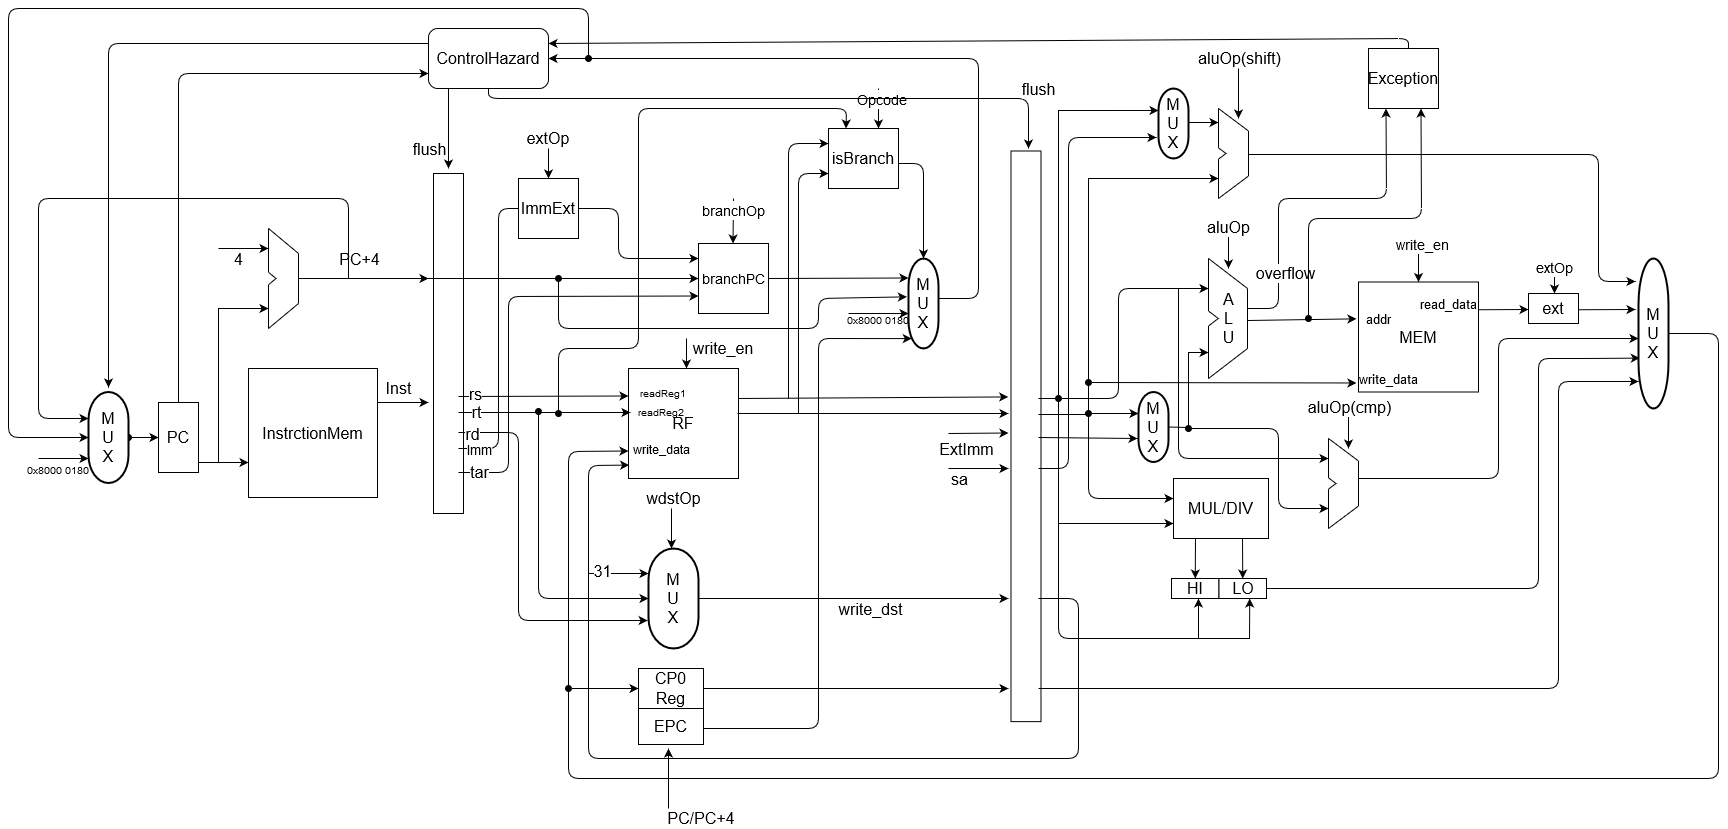
\includegraphics[ width=270mm,center]{3-stages-pipeline.png}
        \caption{三级流水处理器结构图}
        \label{fig:singleblock}
    \end{figure}
    \end{landscape}
\newpage
\section{系统设计} \label{sysdes}%------------------------------
\subsection{System Overview}\label{sub:sysover}
三级流水线处理器的结构图如上图所示
\subsection{数据通路}
\begin{itemize}
    \item{\textbf{取指}\   PC从InstructionMemory从取出指令交给下一个阶段译码。
    而PC可能的取值是PC+4、跳转的地址、异常处理的地址,也有可能来自EPC,因此要用多选器选出PC的值,再从InstructionMemory中取出指令}
    \item{\textbf{译码}\  在这一阶段,需要将执行指令时可能用到的数据准备好,对立即数进行扩展等。另外,因为第三阶段的数据通路比较长,所以可以将判断是否跳转放到译码阶段,尽可能更早知道是否要跳转}
    \item{\textbf{执行访存和写回}\ \  在执行指令时,可以把运算分为移位、算术逻辑运算、比较运算,以及乘除法;在访存时,
    访存的地址一定是来自算术运算的结果,写入的数据是rt的值;对于
    写回,写回寄存器的数据是来自执行和访存的输出,或者是HiLo寄存器}
    % \item{\textbf{使用Chisel3描述结构} Chisel是一种强大的结构化硬件描述语言,可以对模块、接口以及操作等进行高效率的描述,与Verilog语言相比较,对电路的结构属性具有更好的封装,对系统的描述更加简化。我们选择Chisel3是因为在Linux系统中,使用Chisel3完全不再依赖工业EDA软件实现电路的逻辑仿真,更有利于学术研究和教学应用。虽然Chisel语法在不同版本差异不大,但是部分修饰符的描述方式仍然具有差别,详细区别请参考: \url{https://github.com/ucb-bar/chisel3/wiki/Chisel3-vs-Chisel2}.}
\end{itemize}
\subsection{控制通路}
控制主要是通过\mintinline{c}{opcode} \ \mintinline{c}{func}解码出来的信号来进行控制的。
对ALU来讲,控制比较有特点,因为将ALU分成了三个功能不同的ALU,所以
总体上可以直接将\mintinline{c}{opcode}段 \ \mintinline{c}{func}段的后三位来进行控制

\subsection{冒险}
\begin{itemize}
    \item{\textbf{数据冒险} \ 可以发现在一般情况下,对于这种三级流水线都不会产生数据冒险}
    \item {\textbf{控制冒险} \ 控制冒险可以分成两类,一个是由于例外造成的,其他情况分成一类。
    第一种在ALU计算得到结果后才能计算出来,第二种在译码时就可以发现}
\end{itemize}

% -----------------------------------BLOCKS DESIGN----------------------------------------
\section{模块详细设计}
\subsection{数据通路相关}
\subsubsection{ImmExt 扩展单元} 
\paragraph{功能描述} 
对16bits立即数进行扩展
\paragraph{接口定义}
\begin{table}[h]
    \centering
    \begin{tabular}{|c|c|c|c|}
        \hline  
        名称 & 位宽 & 方向 & 描述 \\ \hline 
        imm  & 16 & in & 立即数\\ \hline 
        extImm & 32 & out & 扩展后的立即数 \\ \hline
        extOp & 1 & in & 符号还是无符号扩展\\ \hline
    \end{tabular}
    \caption{ImmExt 接口}
\end{table}

\paragraph{逻辑控制}
可以发现,只有逻辑运算时才进行无符号扩展,进一步可以用\mintinline{c}{opcode[3]&opcode[2]}作为extOp
\begin{table}[h]
    \centering
    \begin{tabular}{|c|c|c|}
        \hline
        extOp & 0 & 1 \\ \hline
        扩展  & signed & unsigned \\ \hline
    \end{tabular}
\end{table} \\

\subsubsection{ALU}\label{sub:alu}
\paragraph{功能描述}
\begin{itemize}
    \item \textbf{算术、逻辑运算ALU}\  用来进行算术运算与逻辑运算,处理类似\mintinline{c}{ADD AND}这类指令
    \item \textbf{移位运算ALU}\  用来进行移位运算, 处理类似于\mintinline{c}{SLL SRL} 这类指令 
    \item \textbf{比较运算ALU} \ 用来进行比较, 处理类似于\mintinline{c}{SLT}这类指令
\end{itemize}
\paragraph{接口定义}
\textbf{算术、逻辑运算ALU}
\begin{table}[h]
    \centering
    \begin{tabular}{|c|c|c|c|}
        \hline  
        名称 & 位宽 & 方向 & 描述 \\
        \hline  
        alu\_A & 32 & in & ALU的操作数 \\
        \hline 
        alu\_B & 32 & in & ALU的操作数 \\
        \hline 
        aluOp & 3 & in & ALU控制信号 \\
        \hline
        alu\_out & 32 & out & ALU计算输出 \\
        \hline
        overflow & 1 & out & 整数溢出标志 \\
        \hline
    \end{tabular}
    \caption{ALU接口}
\end{table}

\textbf{移位运算ALU 比较运算ALU}
剩下两个ALU模块的接口是一样的
\begin{table}[h]
    \centering
    \begin{tabular}{|c|c|c|c|}
        \hline  
        名称 & 位宽 & 方向 & 描述 \\
        \hline  
        alu\_A & 32 & in & ALU的操作数 \\
        \hline 
        alu\_B & 32 & in & ALU的操作数 \\
        \hline 
        aluOp & 3 & in & ALU控制信号 \\
        \hline
        alu\_out & 32 & out & ALU计算输出 \\
        \hline

    \end{tabular}
    \caption{ALU接口}
\end{table}

\paragraph{逻辑控制} 
\textbf{算术、逻辑运算ALU} \\
\begin{table}[h]
    \centering
    \begin{tabular}{|c|c|c|c|c|c|c|c|c|}
        \hline
        aluOp & 000 & 001 & 010 & 011 & 100 & 101 & 110 & 111 \\ \hline
        运算  & ADD & ADDU & SUB & SUBU & AND & OR & NOR & XOR \\ \hline
    \end{tabular}
    \caption{ALU控制}
\end{table} \\
ALU的两个操作数一个是来自rs,一个来自rt或者立即数。用\mintinline{c}{opcode[5:3]}来选择
\begin{minted}{c}
    if opcode[5:3] == 000 :
        alu_B = R[rt]
    else :
        alu_B = extImm 
\end{minted}

\textbf{移位运算ALU} \\
\begin{table}[h]
    \centering
    \begin{tabular}{|c|c|c|c|c|c|c|c|c|}
        \hline
        aluOp & 000 & 001 & 010 & 011 & 100 & 101 & 110 & 111 \\ \hline
        运算  & SLL & xxx & SRL & SRA & SLLV & xxx & SRLV & SRAV \\ \hline
    \end{tabular}
        \caption{ALU控制(xxx是不关心的情况)}
\end{table}\\
这些移位指令都是R-type指令,ALU的操作数alu\_B来自rt,alu\_A来自R[rs]或者sa
\begin{minted}{c}
    alu_A = func[3] ? R[rt] : sa
\end{minted}

\textbf{比较运算ALU} \\
\begin{table}[h]
    \centering
    \begin{tabular}{|c|c|c|c|}
        \hline
        aluOp & 010 & 011 & other\\ \hline
        运算  & signed cmp & unsigned cmp  & xxx \\ \hline
    \end{tabular}
        \caption{ALU控制(xxx是不关心的情况)}
\end{table}\\
ALU的操作数和算术逻辑ALU的操作数一致

\subsection{控制模块}\label{sub:ctl}
\subsubsection{功能描述}
\subsubsection{接口定义}
\subsubsection{逻辑控制}

\subsection{数据通路}\label{sub:dat}
\subsubsection{功能描述}
\subsubsection{接口定义}
\subsubsection{逻辑控制}

%add more subsections for other block in you CPU design.

\section{实验过程记录}\label{labrec}
记录实验的过程,完成了什么样的工作,存在的问题包括哪些,解决方案如何等。subsubsection名称自行设定。

% -----------------------------------Appendix----------------------------------------
\appendix
% \section{代码}\label{sub:app.code}
% 请在附录\ref{sub:app.code}中添加代码。请使用如下Scala的语法高亮描述方法。

\newpage
% -----------------------------------REFERENCE----------------------------------------
\begin{thebibliography}{9}
\bibitem{Erdos01} P. Erd\H os, \emph{A selection of problems and
results in combinatorics}, Recent trends in combinatorics (Matrahaza,
1995), Cambridge Univ. Press, Cambridge, 2001, pp. 1--6.
\end{thebibliography}
\end{document}

